\section{Overview}

My capstone is now a study of how honest the uncertainty around a glucose forecast is. A forecaster predicts glucose 60 minutes ahead, and a band around the forecast tells the person how far to trust it. An 80\% band is honest if the true value falls inside it 80\% of the time. The question I am answering is whether the band stays honest where it matters: in each situation (the current glucose level plus the direction it has moved over the last 30 minutes), for each patient, and on each day (Figure~\ref{fig:axes}). I tested this on 215 patients from 11 public studies. Three studies were used to design the methods. The other eight (153 patients) were held out and used only to check them.

This is not where my Project Brief pointed. On September 26 I proposed continuing GLIMMER \parencite{glimmer2026}, a study that weights a forecaster's mistakes in dangerous glucose ranges more heavily. The following sections explain how I got from there to here: the turns and dead ends (Navigation), how I defined success before each test (Outcome Analysis), how the work compares with professional practice, how I used generative AI, how I used feedback, and what remains before the Full Draft. The work product reports the results; this document is about how I reached them.

Three parts of the process are the ones I am proudest of. The first is a written research protocol (October 17, 2026). Before any test runs, I record the claim, the measure and the threshold for success in the hypothesis register, which is kept in the project repository, and the threshold cannot move afterwards. The register now holds 85 hypotheses. Of these, 36 were not supported and five more were invalidated, and I kept every one. The second is external validation. A result counts as a main finding only if it holds on studies never used to design the method. Those studies cover closed-loop systems (a pump that adjusts insulin automatically from the sensor) and other pumps, children and adults, and three sensor brands \parencite{metabonet2026}. The third is catching my own errors. I found a seed bug in September, test data in an alarm threshold in early October, and mislabeled patients in mid-October. Each was found because I re-checked results before relying on them, and each is described below.

\begin{figure}[htbp]
\centering
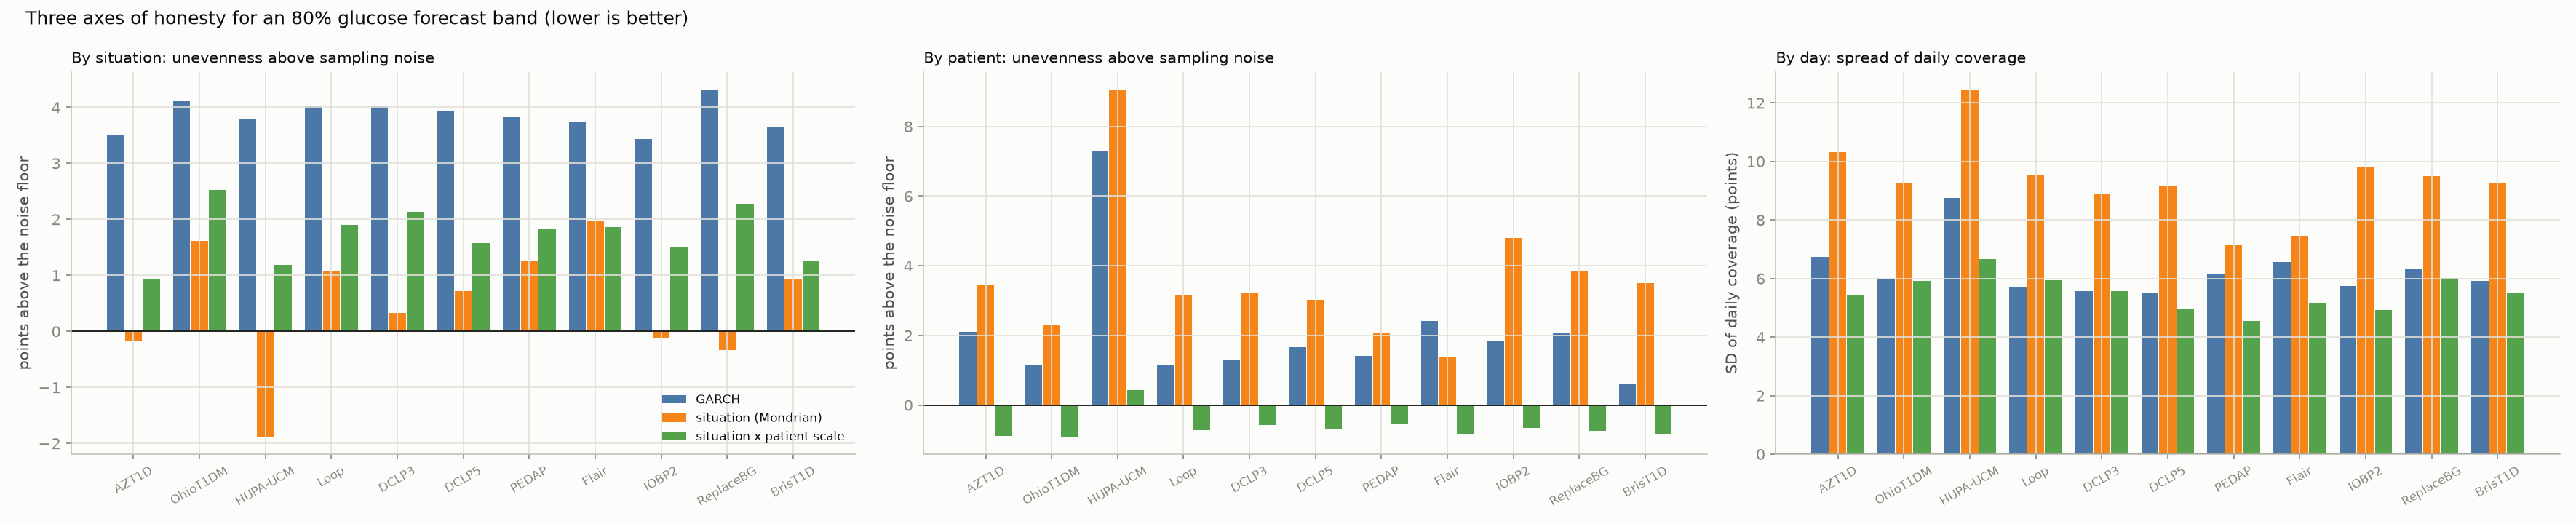
\includegraphics[width=\linewidth]{figures/paper_fig2_three_axes.png}
\caption{The three ways a forecast band can be honest or not: by situation, by patient, and by day.}
\label{fig:axes}
\end{figure}

\section{Navigation: How the Work Moved}

This section follows the project from my choice of topic in early September to the research program I run now. It records the turns, the dead ends and the mistakes, because each one changed what I did next.

\subsection{Starting Point and the GLIMMER Replication}

In early September I sent Prof.\ Watson an idea document with two options. The first was to extend a study on predicting blood glucose for people with diabetes, which fit my Data Science with Machine Learning track. The second was a Zillow-like software product for the Israeli commercial real estate market, which was closer to my career goals but would have meant switching to the software track. I chose the first. Several of my friends have type 1 diabetes, and a model that forecasts glucose an hour ahead gives a person time to act before a high or a low.

The first step was finding data. The standard dataset, OhioT1DM \parencite{marling2020ohio}, requires an access request, and mine went unanswered. Rather than wait, I switched on September 13 to AZT1D \parencite{azt1d2025}, a newer dataset of 25 patients. I later reached OhioT1DM through MetaboNet \parencite{metabonet2026}, a public collection of 14 diabetes datasets, and checked it row by row against AZT1D's own files before relying on it.

I began by replicating GLIMMER, a 2026 study from the group that built AZT1D. It trains forecasters to weight mistakes in dangerous glucose ranges more heavily, and it tunes that weighting for each patient. In my replication, the weighted models caught more dangerous events (the share caught rose from 0.507 to 0.722), but overall accuracy was worse.

On September 15 I found a bug: each patient's weight search had started from the same random seed, so every search was identical. After the fix, the gain from per-patient tuning disappeared (a typical error of 41.12 mg/dL for the tuned model against 41.18 mg/dL for fixed weights). Since then I re-check results before relying on them. After my September 16 presentation, my professor suggested forecasting the whole glucose curve step by step. The curve came out nearly flat, because the model could not predict meals, so on September 19 I set this approach aside. I wrote that day that my next steps were unclear to me.

\subsection{From Forecasting to Uncertainty}

After submitting my Project Brief on September 26, I moved from improving the forecast to estimating how uncertain it is. I borrowed methods from other fields: GARCH \parencite{bollerslev1986garch} and EWMA, which track changing volatility in financial markets; the analog ensemble \parencite{dellemonache2013analog}, which builds a weather forecast from similar past situations; and conformal prediction \parencite{vovk2005alrw}, a statistical method that sizes the band from past errors. Each puts a band around the forecast, and a band that reaches a dangerous level acts as a warning.

The bands failed my first test. Ordinary 80\% and 95\% bands raised alarms on 68\% to 100\% of safe readings. At the same false-alarm rate, the methods caught between 74\% and 76.5\% of dangerous readings, so none was clearly better. On September 28 I wrote in my journal that I did not think I could create meaningful insights without driving the false alarm rate up drastically.

Instead of testing more methods, I looked at where the error comes from. More data would barely help (unlimited data of this kind would cut the error by about 2\%), the model did not degrade over time, and a simple alarm threshold did better than the bands. One map was more useful: the typical error was about 26 mg/dL when glucose was steady between 70 and 180 mg/dL, but 61 mg/dL during a fast rise above 250, and band coverage swung from 64\% to 95\% across these situations. The band was honest on average and dishonest in the situations that mattered. By my October 6 slides, these results had narrowed the work to two avenues.

\subsection{Choosing One Direction}

The first avenue gives each situation its own band. On October 4 I tested it on OhioT1DM, data it was never designed on, with the rule for success written down first. It held: the distance from the 80\% target fell by 41\%, 9 of 12 patients were closer, and the bands were 12\% narrower. A literature check the same day showed that this method already has a name, Mondrian conformal prediction \parencite{vovk2005alrw}, so I reframed the contribution as what the method reveals about glucose forecasts, not the method itself. Other checks that day showed the overall gain was small: the bands became more even across situations, but they did not catch more of the large errors.

The second avenue followed Prof.\ Watson's feedback on my Project Brief and asked what makes a patient hard to predict. I tried an autoencoder (a network that compresses two hours of readings into a few numbers) and a measure of how irregular a glucose record is. Neither showed much beyond the glucose level itself, and on October 6 I closed this line. The details are in the section on feedback. On October 7, at Prof.\ Watson's suggestion, I drew the autoencoder's output with t-SNE, a method that draws many-dimensional data in two dimensions. It showed that the autoencoder had learned level and trend (Figure~\ref{fig:tsne}). This matched the grouping behind the first avenue, but it felt obvious.

\begin{figure}[htbp]
\centering
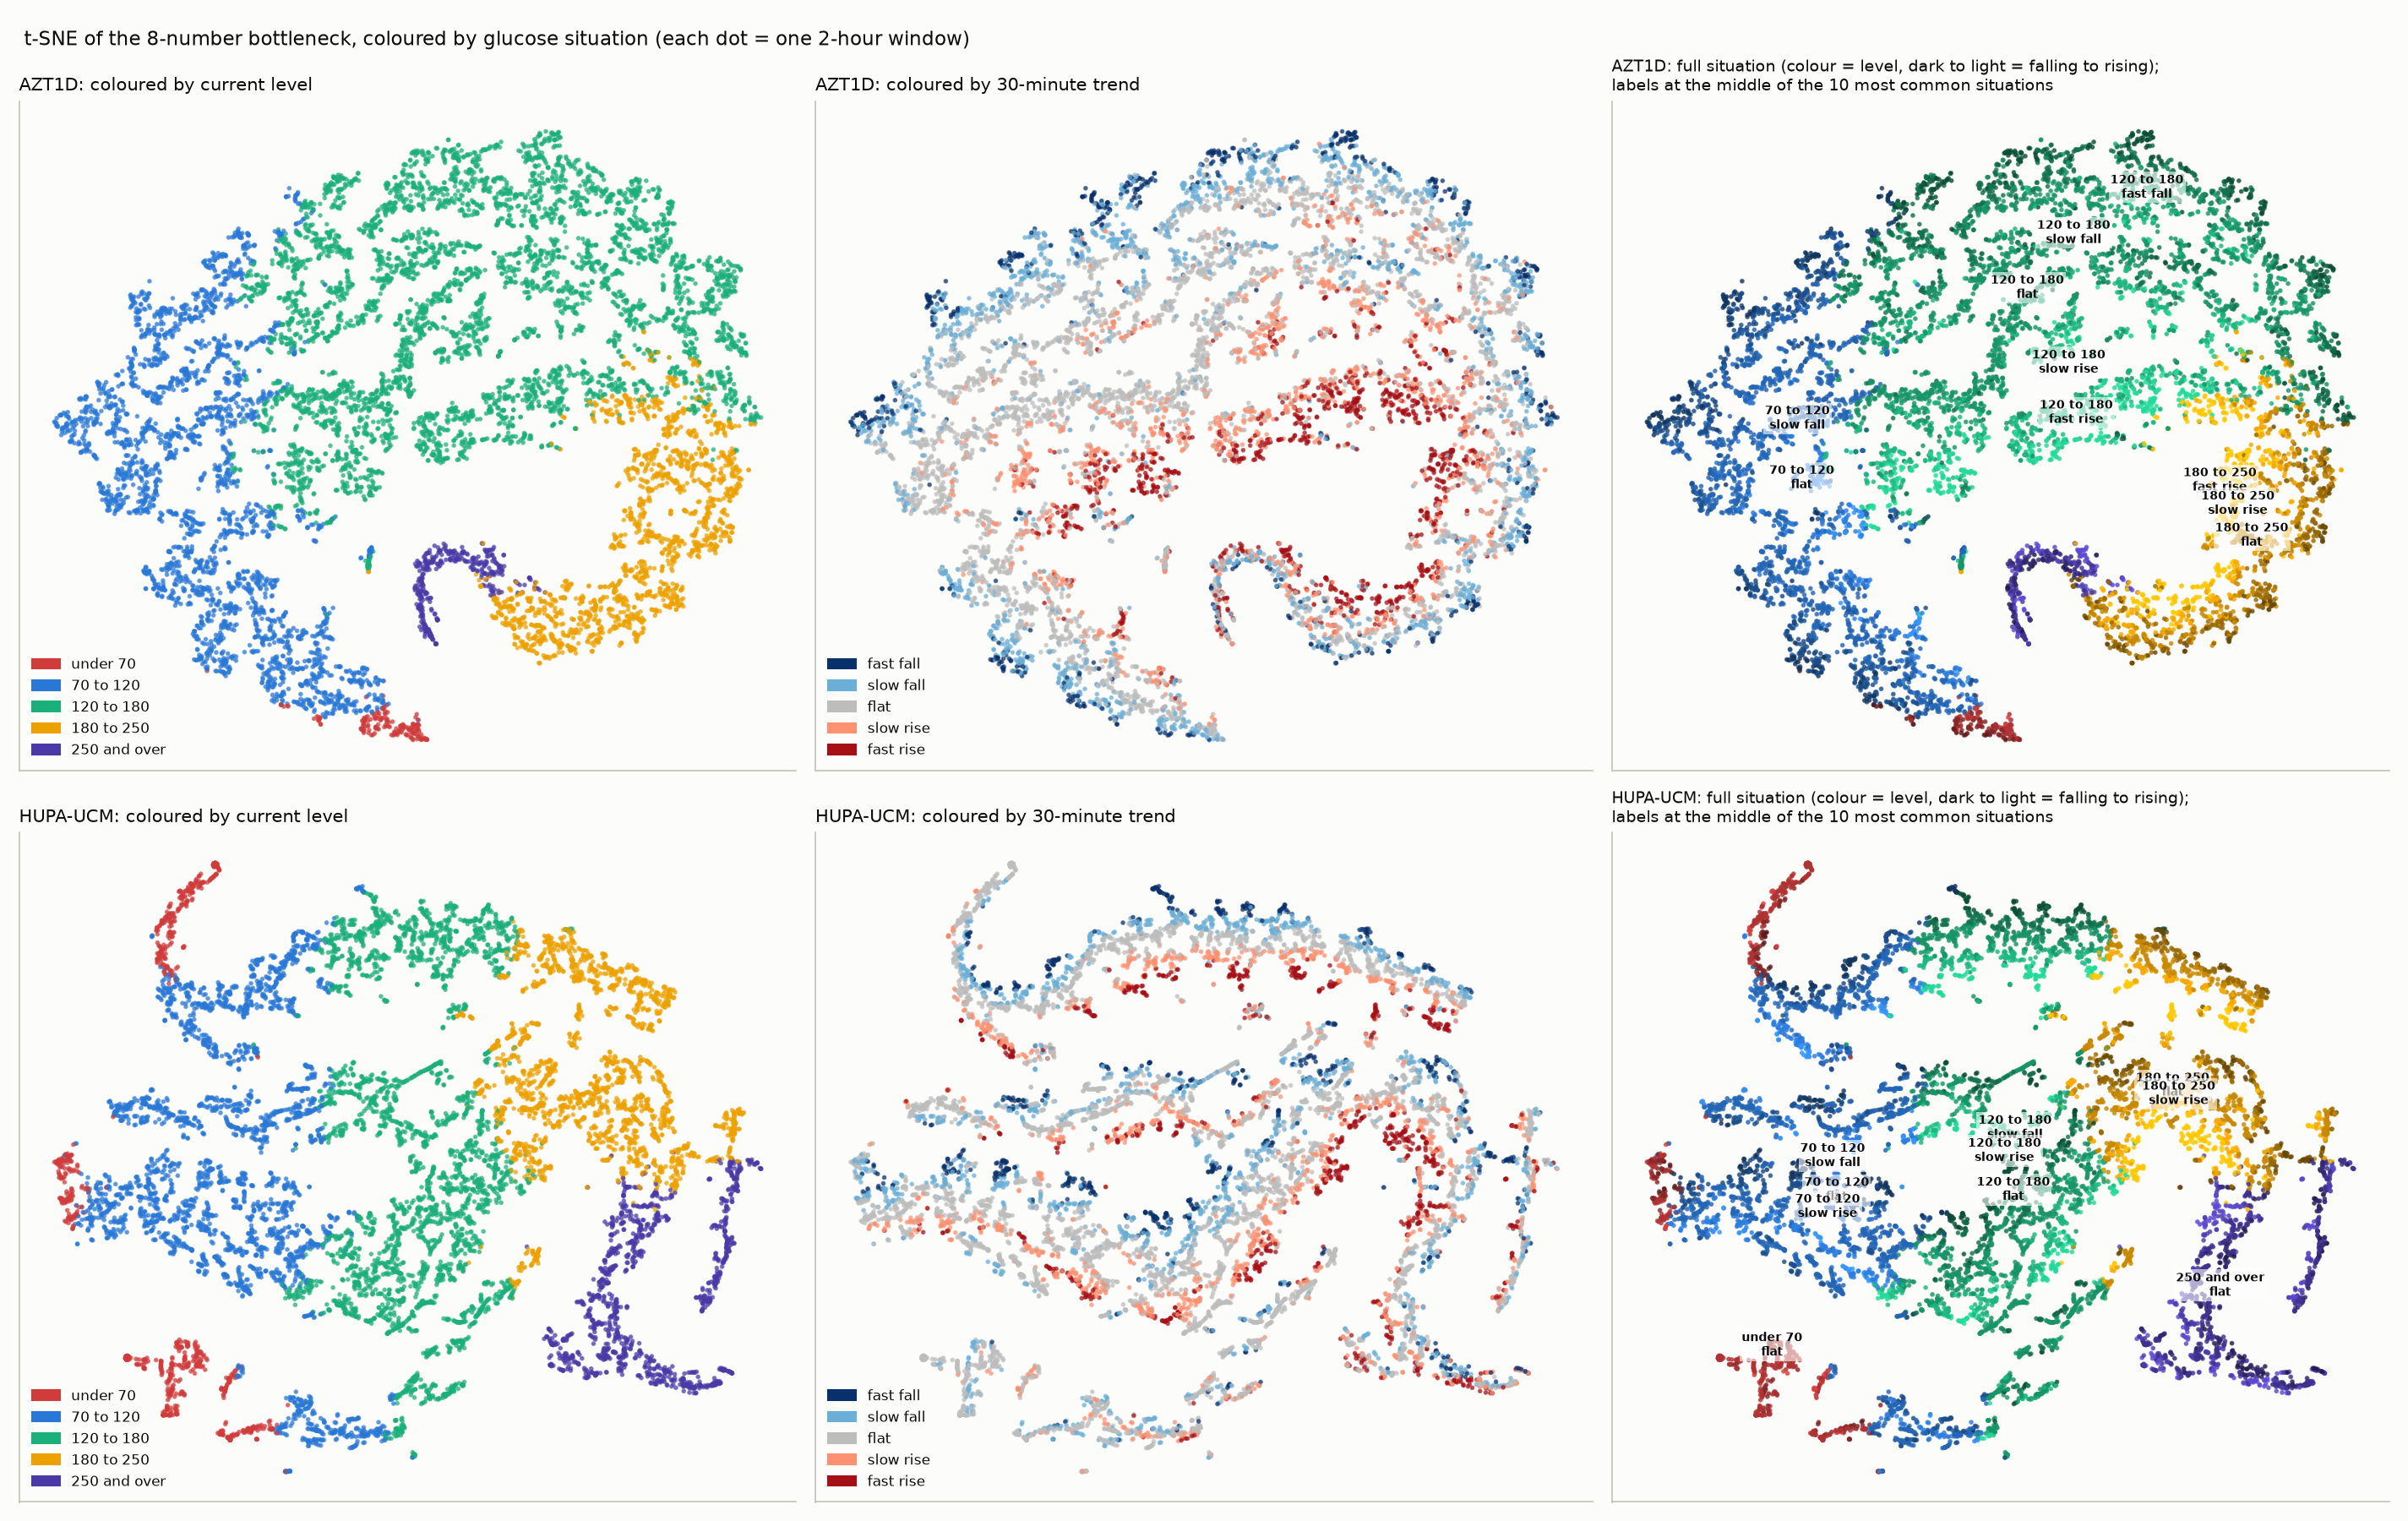
\includegraphics[width=\linewidth]{figures/tsne_situation.png}
\caption{The autoencoder's summary of each two-hour window, drawn in two dimensions and colored by current glucose level, 30-minute trend, and both together. Windows sort by level and then by trend, the same structure as the situation grid.}
\label{fig:tsne}
\end{figure}

My October 6 slides for my second reader, Volkan, put the doubt plainly: ``My concern is that this may not be a valuable avenue. The average stays about the same, and it does not catch more of the large errors.'' At our October 8 meeting, Volkan said the path was good and that it was critical for the findings to have value. That comment framed the next two weeks, as I describe under Feedback.

\subsection{From Exploration to a Research Program}

By mid-October I had many small results and no clear way to know which were real. On October 12 I tried a simulation as an answer key: simulated patients with sensor noise I planted myself, so the true answer was known. The situation bands did worse than GARCH there, but the simulated patients were too easy to forecast (a typical error of 11 to 16 mg/dL, against 31 to 39 mg/dL on real patients), so the test could not settle the question. I left a harder simulator for future work.

On October 17 I wrote the research protocol (work/RESEARCH\_PROTOCOL.md). Its rules are set out in the next section. The same day I let Claude Code run pre-registered tests without checking in with me for each one, since the rules were now written down.

In plain words, the program turned the first avenue into the core of a paper and answered my doubt about its value. The situation bands stayed better calibrated than GARCH in all eight outside studies. I then checked how uneven coverage looks from chance alone, and found that most of the real problem left over was between patients. A per-patient scale, learned from errors seen an hour later while the band is in use, removed it. What makes a patient hard to forecast turned out to be mostly how fast their glucose moves. The protocol also forced cuts. After the fifth design of a band meant to be honest for each patient and each situation at once, I stopped tuning and reported all five.

\subsection{Setbacks and How I Handled Them}

\subsubsection{The Shared Seed}
The seed bug of September 15 surfaced while I was checking results that Claude Code had produced, and it erased the personalization gain. Since then every patient and every ensemble member gets its own seed, and this rule is written into the project instructions the AI reads.

\subsubsection{Test Data in the Alarm Thresholds}
On October 4 the first run of an alarm test tuned its thresholds on the test period, the data meant only for scoring. I retuned on the validation period, and the band alarm still lost. The protocol now lists threshold choice beside fitting and calibration as places test data may never enter.

\subsubsection{A Missing Label That Flipped a Conclusion}
On October 17 I concluded that closed-loop systems made no difference to forecast difficulty. On October 18 a check of the labels behind that result found that 12 of 13 BrisT1D patients had no device label in MetaboNet and had been coded as not closed loop, although several use closed-loop pumps. After correcting them, closed-loop patients were 5.6\% to 6.5\% harder to forecast once glucose variability was accounted for, and the verdict changed. The difference disappeared once I accounted for how fast each patient's glucose moves. I logged this as a correction entry rather than editing the old one, so both versions stay visible.

\subsubsection{An Unfair Baseline}
On October 17 a first comparison used a GARCH band whose scale was off by a constant, and a combined GARCH band that became unstable on HUPA-UCM \parencite{hupa2024}. Beating a broken baseline would have proved nothing, so I fixed both baselines on the validation period and left the tested methods untouched. The log records this as a fix to the baseline, not to the method being tested.

\subsubsection{The Missing Data File}
Around October 18 the 1.3 GB MetaboNet file disappeared from my Downloads folder. A training run stopped after the 25 AZT1D patients, and predictions saved only at the end were lost. I changed the script to save as it goes and skip finished work, and the AZT1D and HUPA-UCM runs finished on October 20. Two optional checks stay blocked until I restore the file (see Next Steps). \todo{TO FILL: whether the MetaboNet file has been restored, and where raw data will live from now on}

\subsection{Planning: The Timeline I Set and What Happened}

On October 4 I sat down to map the fixed points of the course. I drew a square for each remaining week on my iPad, with its deadlines and the deliverables I set for myself, and filled in the first four (Figure~\ref{fig:ipadplan}). I also drew a task list for that day (Figure~\ref{fig:ipadtasks}). The handwriting was too slow and could not be read by AI, so I rebuilt it as a Notion Gantt. The course deadlines on it are the Second Reader meeting (October 8), the Midterm (October 31), the Second Presentation, a go or no-go decision (November 20), and the Full Draft (December 11). Table~\ref{tab:planactual} compares the October 4 plan with what happened.

\begin{figure}[htbp]
\centering
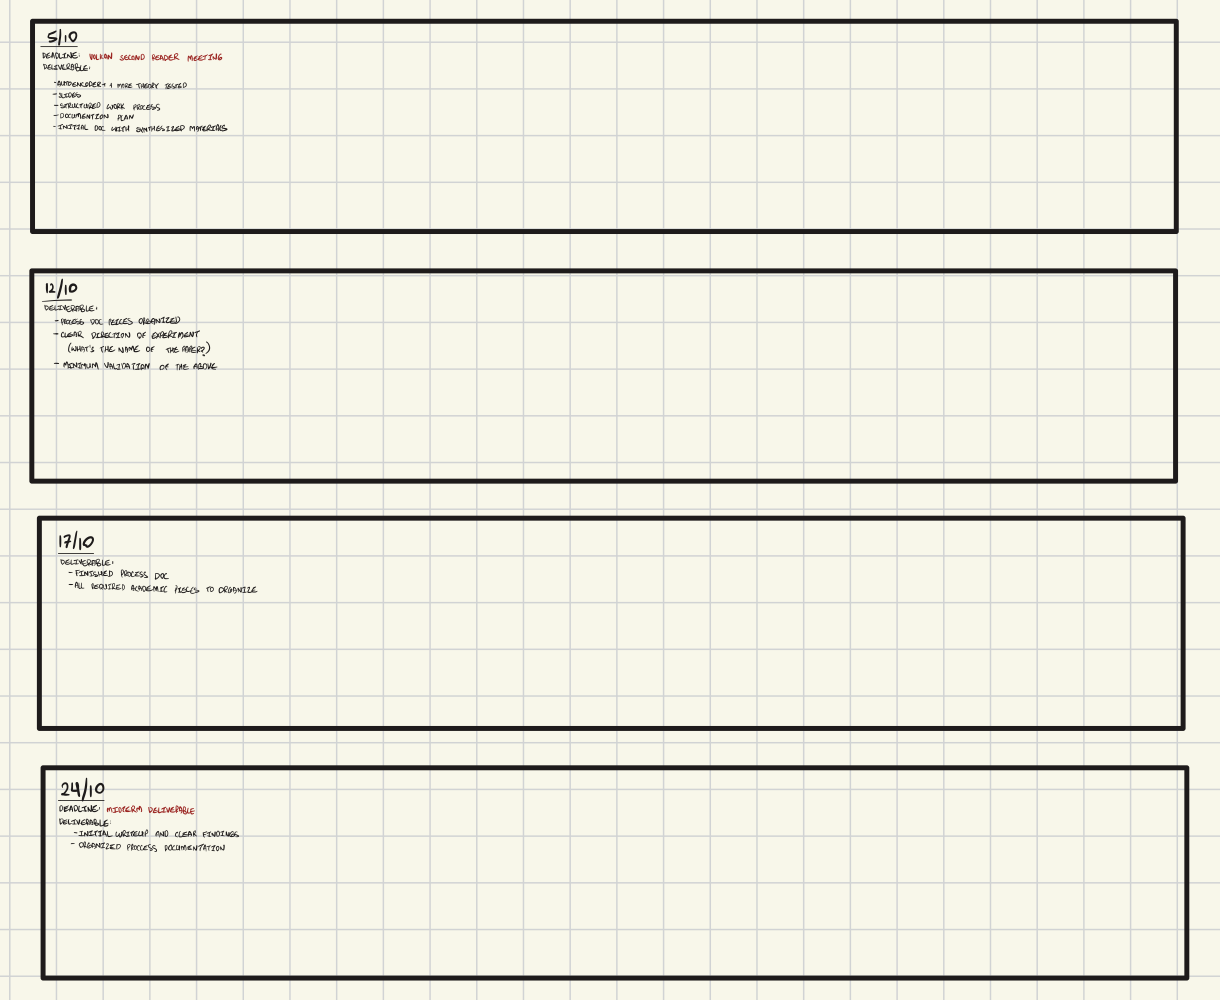
\includegraphics[width=\linewidth]{figures/ipad_week_plan_oct4.png}
\caption{My hand-drawn plan from October 4, 2026: one square per remaining week, with course deadlines and my own deliverables for the first four weeks.}
\label{fig:ipadplan}
\end{figure}

\begin{figure}[htbp]
\centering
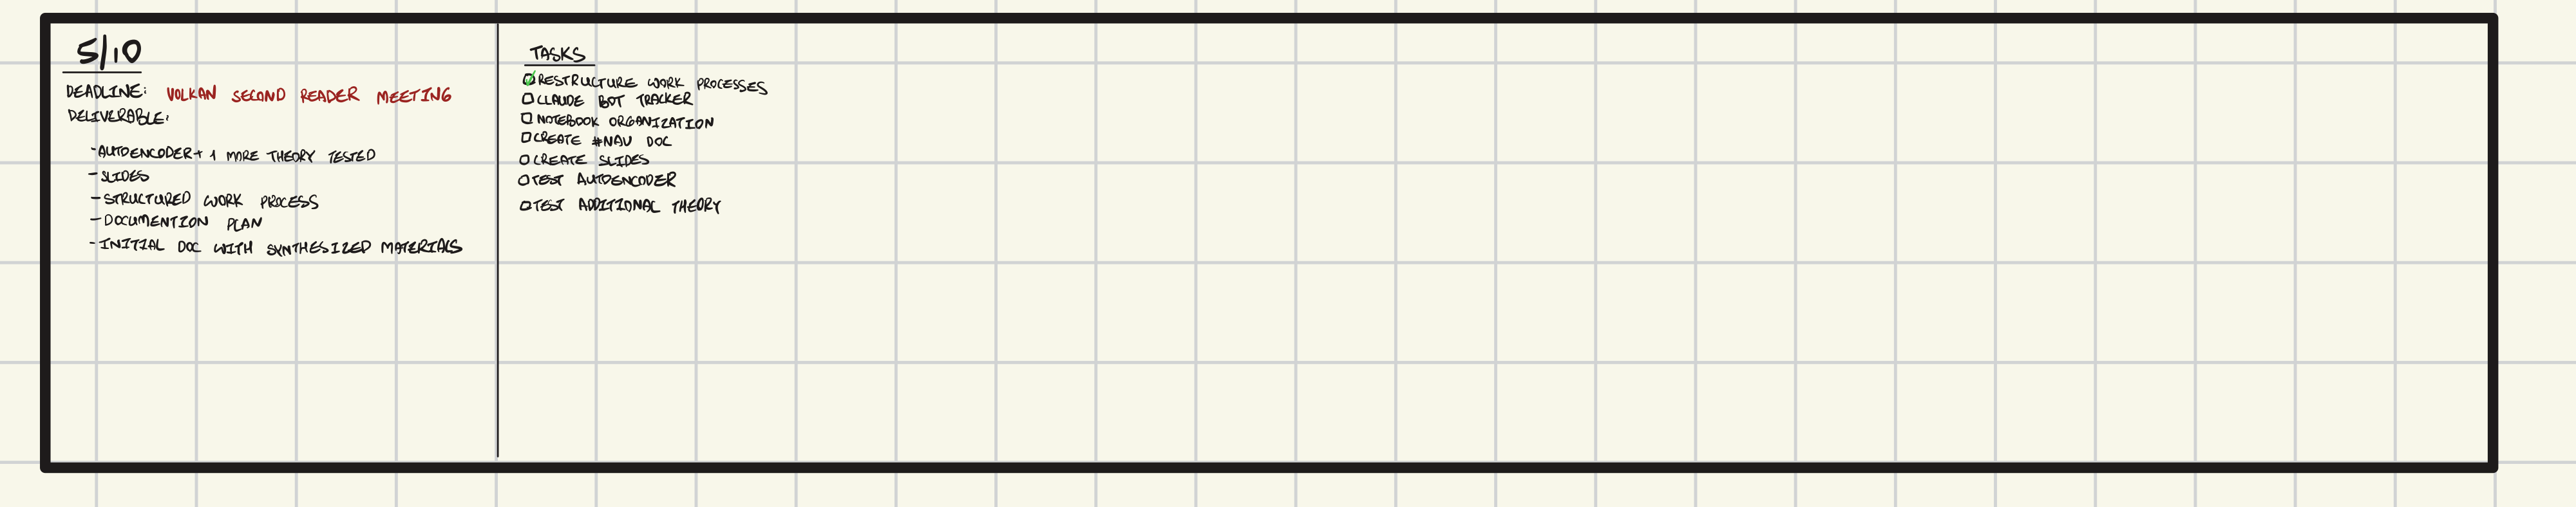
\includegraphics[width=\linewidth]{figures/ipad_task_list_oct4.png}
\caption{My hand-drawn task list for October 4, 2026, the day I reorganized the project.}
\label{fig:ipadtasks}
\end{figure}

\begin{table}[htbp]
\caption{Deliverables I Planned on October 4 Compared With What Happened}
\label{tab:planactual}
\small
\begin{tabular}{p{0.12\linewidth}p{0.38\linewidth}p{0.42\linewidth}}
\hline
Week of & Planned & What happened \\
\hline
Oct 5 & Autoencoder and one more theory tested; slides; structured work process; documentation plan; first document of synthesized materials & Autoencoder and entropy tested, then closed on October 6; slides ready for the October 8 meeting \\
Oct 12 & Process documentation pieces organized; a clear direction (``what's the name of the paper?''); minimum validation & Direction and validation went beyond the plan: the research protocol and tests on 11 studies; process pieces not yet organized \\
Oct 17 & Finished process documentation; academic pieces organized & A paper draft built from the findings on October 17; research and corrections continued; the data file loss stopped one run; process documentation slipped \\
Oct 24 & First write-up with clear findings; organized process documentation & Organization map and Midterm structure on October 25; this document in progress \\
\hline
\end{tabular}
\end{table}

The pattern is clear. The research ran ahead of the plan, and the documentation fell behind it. \todo{TO FILL: how I plan to rebalance research and writing between now and the December 11 Full Draft}

\subsection{Working Habits and Tools}

I block 7:30 to 9:30am for the capstone. On October 3 I noticed that I skipped this window on certain days, and I listed three options: accept three days a week, wake up earlier on Wednesdays, or move those sessions to the evening. I chose the earlier wake-up, with the evening as a fallback and three days as a last resort. On October 12 I wrote that the morning block had let me push forward at a consistent rate. On September 22 I realized that Prof.\ Watson had wanted something different from what I had done, so I decided to follow Slack more closely, with a daily reminder.

On October 4 I reorganized my files into one folder per week, each with a short summary of its hypotheses, findings and open items. My Notion journal holds dated reflections from September 10 onward, and the Gantt holds the plan. Code, results and figures are backed up to a public GitHub repository, with every unit of work in a work log. On October 3 I wrote that my failed experiments would be as much a part of the capstone as the results that work, and these records exist so that the failures stay visible.

\section{Outcome Analysis: Defining Success Before Running}

From early October I wrote down a rule for success before each test. The seed bug had shown me how easily a result can look like a finding when it is not one. On October 17 I made this stricter with the research protocol, so that every test for the paper had a numeric rule saved before it ran. This section sets out the success criteria for this deliverable, the rules I used to decide whether a test passed, and an honest count of how the tests turned out.

\subsection{Success Criteria for This Deliverable}

I propose four criteria for judging the work so far. Each is something an outside reader can check. \todo{TO CONFIRM: these four success criteria}

\begin{enumerate}
\item \textbf{The main claim holds on data never used to design it.} Met. The main claim is that sizing the band separately for each situation keeps it close to its stated coverage in each situation, not just on average. I tested it on eight MetaboNet studies that I had not used while building the method, and it held in all eight (see the worked example below).
\item \textbf{Every number traces to a saved result file.} Mostly met. The project rules I wrote for the AI say to report numbers only from outputs shown in a session or from saved result files, and most rows of the hypothesis register link to the result file behind them. A few rows do not, and I have not yet checked every number in the paper draft by hand, so this needs a final audit before the Full Draft.
\item \textbf{Failed tests are reported, not hidden.} Met. Every test stays in the hypothesis register whatever its outcome. The paper supplement copies these rows, but it was made on October 17 and does not yet include the tests added after that, so I need to update it.
\item \textbf{The method beats strong standard baselines, not weak ones.} Partly met. I compared my band with two standard methods. The first uses deep ensembles \parencite{lakshminarayanan2017ensembles}, several networks trained with different random seeds whose disagreement sets the band. The second is a network that predicts its own band and is then corrected with conformal prediction \parencite{romano2019cqr}. My band was more even across situations and across patients on the two datasets where the comparison could run; the third was blocked by the missing data file. On one dataset the second method gave a slightly better combined score of width and misses, and a richer version of it produced sharper bands than mine, though less even ones. So my method does not win on every measure.
\end{enumerate}

\subsection{Pre-Registration and Evidence Tiers}

Pre-registration means writing down the rule for success before running the test. For every test in the paper, I added a row to the hypothesis register with the claim, the measure, the threshold that counts as success and the data it would run on. I then committed that row to version control (git), which records the time of every change. Because the rule is time-stamped before the result, anyone can check that I did not choose the threshold after seeing the answer.

The rules never moved after a run. If a test failed and I thought of a better design, I wrote it up as a new hypothesis and labelled it as a second, third, fourth or fifth try. A line of work stops after two pre-registered failures in a row with no new mechanism to test, and I do not keep tuning a method until it wins. One verdict did change, for a different reason: the closed-loop test described under Setbacks failed, then passed after the labels were corrected. The register keeps both versions and the reason.

The protocol sorts results into four evidence tiers, which decide where a result can appear in the paper:

\begin{itemize}
\item \textbf{Look:} a picture or a number with no rule set beforehand. At most a motivating figure.
\item \textbf{Preliminary:} pre-registered, but on one dataset or one random seed. Discussion only, as a lead.
\item \textbf{Replicated:} holds on at least two independent datasets, and a confidence interval built by resampling patients excludes no effect. Results section.
\item \textbf{Paper-grade:} replicated, and also holds on outside data never used to design the method, and survives changes to the main analysis choices. Only these results go in the abstract.
\end{itemize}

A worked example shows how this played out. On October 17 at 9:01pm I committed the rule for the external test: across eight outside studies of about 20 patients each, the situation bands had to be at least 20\% more even across situations than GARCH in at least six of the eight. Here ``even across situations'' means how far, on average, the share of readings inside an 80\% band is from 80\% within each situation. The result was committed at 9:38pm. The situation bands passed in all eight studies, covering 153 patients. Their average gap was 2.25 to 4.19 percentage points, against 5.48 to 6.76 for GARCH (Figure~\ref{fig:external}). This moved the main finding to the paper-grade tier.

\begin{figure}[htbp]
\centering
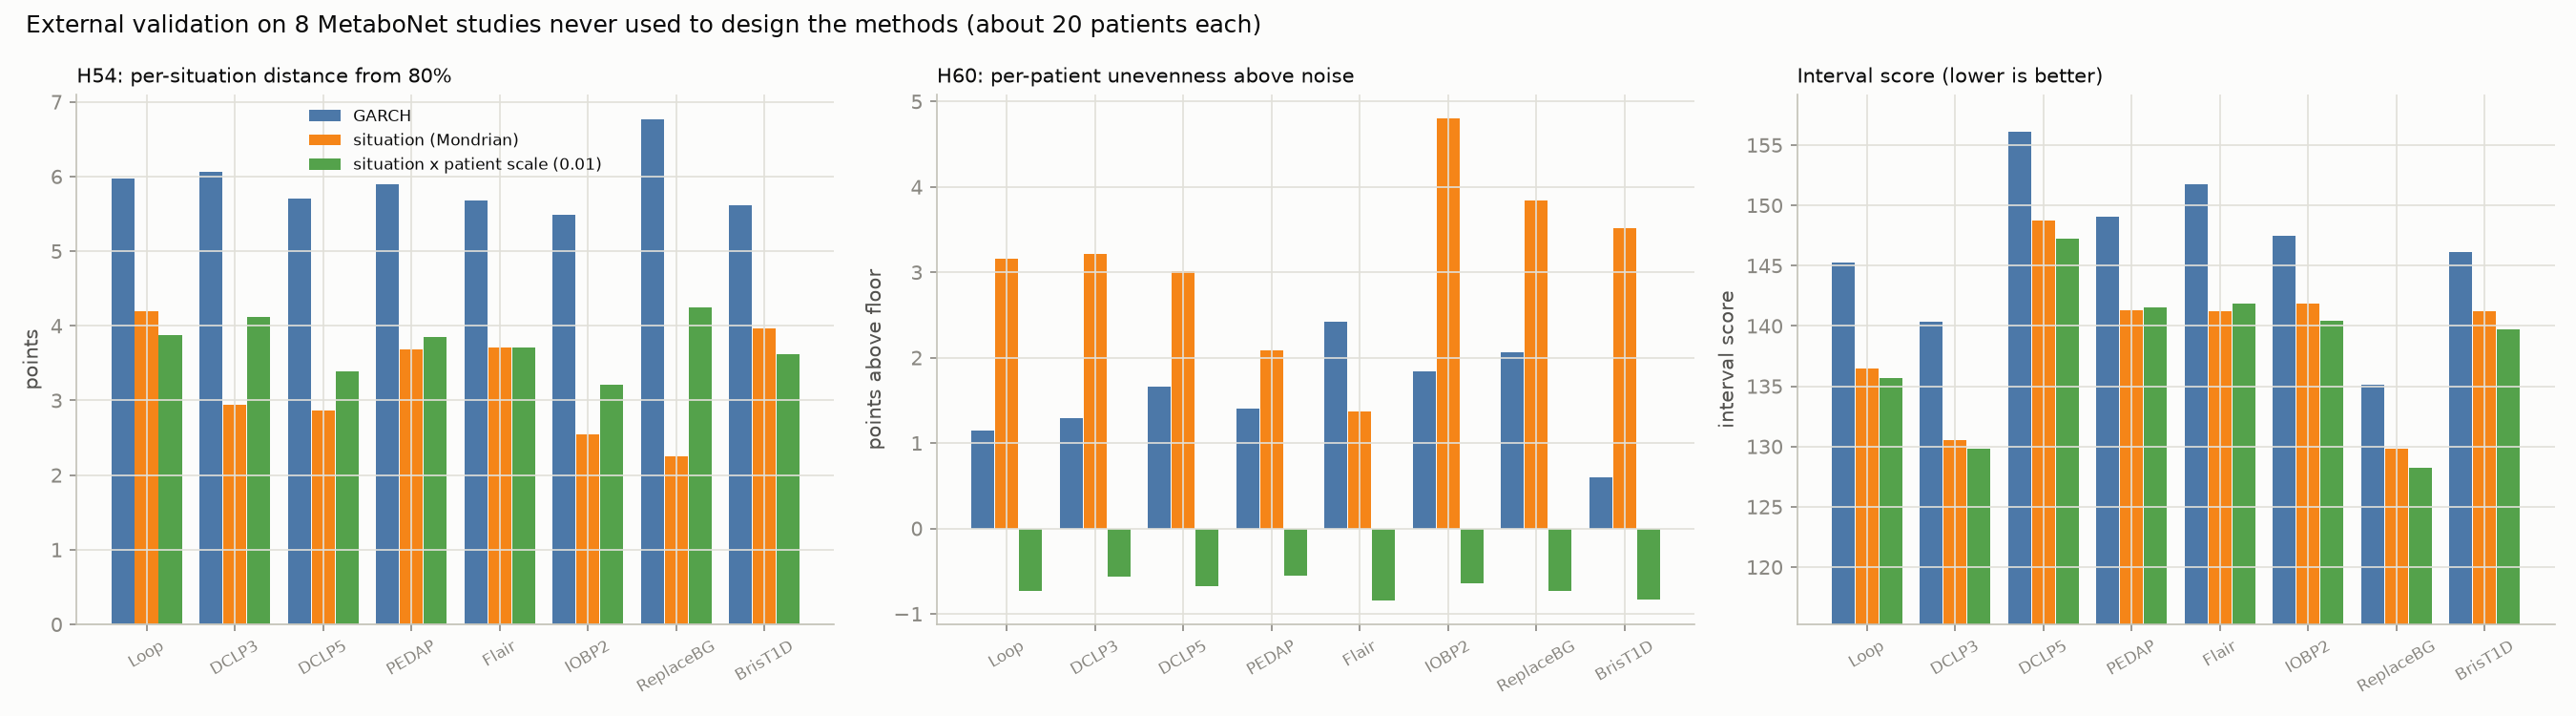
\includegraphics[width=\linewidth]{figures/h54_panel_external.png}
\caption{External test on eight MetaboNet studies that were never used to design the methods. Left: how far each method's 80\% band is from 80\% within each situation (lower is better). Middle: how uneven the band is across patients beyond what chance alone would produce. Right: a combined score of band width and misses (lower is better).}
\label{fig:external}
\end{figure}

\subsection{Self-Assessment}

On October 17 and 18 I pre-registered 38 tests for the paper. One was confirmed, 19 were supported, 17 were not supported, and one is still being tested. Several of the supported results carry a qualification: two passed on two of three datasets, one passed only on the two datasets that were available, one depends on an assumption about sensor error, and one passed only after the label correction. I count the 17 failures as part of the work. They showed me that some fixes for one kind of unevenness make another kind worse.

The evidence is still weak in three places. First, on OhioT1DM the situation bands keep a small amount of unevenness across situations beyond chance. A second training seed gave the same result, so this is likely real. Second, most forecasters were trained with one seed per patient, and the outside studies were not retrained with a second seed. Third, the missing MetaboNet file blocks two optional checks.

There is also a question about pace. I pre-registered 38 tests in two days, and ran most of them in that time, because Claude Code carried out each round against the protocol. \todo{TO FILL: how I reviewed these rounds and what I checked myself before accepting a verdict}

\section{Modeling Professional Process}

Good practice in machine learning for health has a few common parts. Studies pre-register their analysis so that thresholds are not chosen after the fact \parencite{nosek2018preregistration}. They test a model on outside data, since a model that works on the patients it was built on often does worse on new ones \parencite{collins2024tripodai}. They compare against strong, standard baselines rather than weak ones. They report null results and share code.

This project followed most of these. Rules were committed before each run, and the main claim was tested on eight outside studies. The methods were called by their standard names, such as Mondrian conformal prediction \parencite{vovk2005alrw} and adaptive conformal inference, which adjusts the band as new errors come in \parencite{gibbs2021aci}. Every null result stays in the register, and the code, results and figures are in a public repository.

The project departed from usual practice in four ways. First, pre-registration lived in my own repository, not in a public registry. Git time stamps give a weaker but checkable version. Second, Claude Code wrote most of the code, which the next section addresses. Third, I trained one forecaster per patient, following GLIMMER, while a deployed product would more likely use one shared model. I tested a shared model on patients it had never seen. The patient-level fix still held, but the situation results weakened on two of three datasets. Fourth, there is no clinical outcome: the work measures whether bands are honest, not whether they help patients make better decisions. That would need a clinical study, which is beyond a capstone.

\section{Use of Generative AI}

Claude Code, an AI coding assistant made by Anthropic, writes most of my code. I decide what to test and check what comes back. That split has held since my first week, when I wrote in my journal that I was working ``more as a validator than anything else'' while I replicated GLIMMER. What changed over the semester is how much the assistant does on its own. Until October 17, it asked me before any run longer than 10 minutes. On October 17 I let it work on its own under the research protocol, with no check-ins and no limit on run time, and it has since tested 38 hypotheses this way. The checks below matter more now than they did in September.

\subsection{What the AI Did and What I Decided}

The assistant wrote the data loaders, the forecasting models, the uncertainty methods and the scripts that score them. It ran the training jobs, saved the results to files and wrote a first reading of each result. I chose the topic, the datasets and the questions, I set what counts as success, and I made the calls to change direction, such as closing the autoencoder line on October 6. Table~\ref{tab:ai-roles} summarizes the split.

\begin{table}[htbp]
\caption{Who Did What in the Project}
\label{tab:ai-roles}
\begin{tabular}{p{0.24\linewidth}p{0.34\linewidth}p{0.34\linewidth}}
\hline
Task & Claude Code & Me \\
\hline
Choosing questions & Proposes next questions under the protocol (since October 17) & Chose the topic, the datasets and every change of direction \\
Defining success & Writes the rule into the register before a run & Set the protocol that requires a rule before every run \\
Writing code & Wrote most of the code & Reviewed it and asked for checks \\
Running analyses & Ran training jobs and saved results & Approved long runs until October 17 \\
Judging results & Gives a first verdict against the rule & Read the figures and made the final call \\
Keeping records & Writes work log entries & Daily summaries and the Notion journal \\
\hline
\end{tabular}
\end{table}

\subsection{How I Checked the AI's Work}

An assistant that writes code quickly can also produce wrong results quickly, and a wrong result can look convincing. I relied on four safeguards beyond the pre-registration described above. First, I wrote the rules the assistant works under into a file called \texttt{CLAUDE.md}, which it reads at the start of every session. Second, every number in my writing must come from an output shown in a session or from a saved result file. Third, the work log records every unit of work, and a mistake is fixed with a new correction entry that names the entry it corrects, rather than by rewriting the old one. Fourth, \texttt{CLAUDE.md} holds a list of traps already hit: a shared random seed, test data leaking into fitting, and one patient making up 53\% of the readings in a pooled dataset. It also requires that results from one seed or five patients be called preliminary. These rules apply to baselines too, which is why the unfair GARCH baseline was fixed rather than beaten.

\subsection{Annotated Examples}

\subsubsection{The Seed Bug}

\textit{What happened.} Before the September 15 fix, per-patient tuning seemed to lower the typical error from 41.18 to 37.44 mg/dL. After each patient got its own seed, the error was 41.12, and the gain was gone.

\textit{Commentary.} The code ran without errors and the result looked like a success. It was simply wrong. This is why ``each patient needs its own seed'' is the first item on the traps list. \todo{TO FILL: how I noticed the seed bug, and how it felt to lose the result}

\subsubsection{The BrisT1D Label Correction}

\textit{What happened.} The closed-loop result described under Setbacks flipped because of 12 missing device labels, not because of a coding error.

\textit{Commentary.} The error was in the data labels, which had been taken as given. The check ran during the assistant's autonomous work. \todo{TO FILL: who spotted the missing labels, and what it taught me about trusting dataset labels}

\subsubsection{Stopping After Five Designs}

\textit{What happened.} In mid-October I wanted a band that is honest for each patient and for each situation at the same time. The assistant tried one design, then another, and each try was recorded in the register as the second, third, fourth or fifth design. On October 18 the fifth design failed its rule, and tuning stopped there, as the protocol requires.

\textit{Commentary.} With an assistant, a sixth and seventh try cost almost nothing, and that is the risk: with enough tries, a method will beat a baseline by chance. Reporting the number of tries keeps the claim honest. \todo{TO FILL: whether I was tempted to continue, and why stopping felt right or wrong}

\section{Feedback and How I Used It}

Prof.\ Watson's feedback on the Project Brief made three research suggestions, and I tested each one. He suggested approximate entropy \parencite{pincus1991apen} to capture major shifts. I tested sample entropy, a close relative that measures how irregular a glucose record is \parencite{richman2000sampen}. It improved the prediction of a patient's forecast error by 9\% beyond how variable their glucose is, short of the 15\% I had set in advance. He also suggested autoencoders. Mine did not reveal anything beyond glucose level, trend and variability, which is why I closed that line on October 6. When I returned to it on October 17, glucose level and trend explained 87\% of what the autoencoder kept, and the small remainder did not help predict how wrong a forecast would be. Finally, he noted that most major changes come from eating and insulin, and that subtler drivers would be worth knowing about. For new patients, meals and insulin explained almost none of that remainder. The subtler driver turned out to be how fast a patient's glucose moves, which explains more than half of why some patients are harder to forecast than others.

Volkan's comment on October 8, that the findings must have value, matched the doubt I had written on my own slide (quoted in the Navigation section). In the weeks after, I wrote the protocol so that no finding counts as a main result until it holds on studies never used to design it. \todo{TO FILL: how Volkan's comment on value changed what I chose to test in the week of October 12, in my own words}


\section{Habits of Mind and Learning Outcomes}

This section lists the learning outcomes and habits of mind (HCs) used in this deliverable, each tied to a moment described above.

\subsection{Capstone Learning Outcomes}

\begin{description}
\item[\#navigation] I closed the autoencoder line on October 6 when it gave no insight, and I reorganized my files and planning in early October.
\item[\#outcomeanalysis] Every hypothesis had a success rule before its run; 36 of 85 were not supported and stay on record.
\item[\#qualitydeliverables] I wrote this document in LaTeX in APA style, with every number checked against saved files.
\item[\#curation] Each dataset is cataloged with its source, license and import date, and the work is filed in one folder per week.
\end{description}

\subsection{Major Learning Outcomes}

\begin{description}
\item[\#cs156-MLCode] I replicated per-patient forecasting networks and fixed the shared-seed bug in the weight search.
\item[\#cs156-MLExplanation] In my second-reader slides, I explained in plain words what the autoencoder was meant to show, and later why it did not show enough.
\item[\#cs166-EmpiricalAnalysis] I used simulated patients with planted sensor noise, and shuffled the situation labels to check that a gain did not come from splitting the data alone.
\item[\#cs114-ModelSelection] I compared band methods at matched false-alarm rates and tested whether a coarser or finer situation grid changed the result.
\item[\#cs110-CodeReadability] Shared code sits in one library, and project rules fix how scripts find files.
\end{description}

\subsection{Habits of Mind}

\begin{description}
\item[\#hypothesisdevelopment] The protocol requires each question to be one sentence about a quantity that can be measured.
\item[\#testability] Each rule names a metric and a threshold, so a result can clearly fail.
\item[\#gapanalysis] I record a gap as ``not found in a stated search'' and log the searches; one gap that came from AI research still needs my own confirmation.
\item[\#studyreplication] I began by replicating GLIMMER, and the protocol says to replicate before extending.
\item[\#dataviz] Figures are read before results are written, and paper figures are titled by the question they answer.
\item[\#confidenceintervals] Intervals come from resampling whole patients, since readings from one patient are not independent.
\item[\#sampling] I treat the patient as the unit, and tested the main finding on 153 patients from eight studies never used to design it.
\item[\#biasidentification] I caught one patient making up 53\% of a dataset, and the mislabeled BrisT1D patients.
\item[\#organization] I work from 7:30 to 9:30am with fallbacks, and keep weekly folders and a work log.
\item[\#professionalism] After I misread what Prof.\ Watson wanted in September, I set a daily reminder to check Slack.
\item[\#audience] I wrote the second-reader slides and this document for non-specialists, explaining each method in plain words.
\end{description}

\section{Next Steps Toward the Full Draft}

The Full Draft is due December 11, 2026. Most of the remaining work is writing. The paper draft already has the abstract, introduction, data and methods. What remains is to write the results and discussion around the main finding: an honest band needs a fixed adjustment for the situation and a slow adjustment for each patient, learned while the band is in use. I am also moving the writing from Google Docs to LaTeX, which handles the structure of a paper better and is easier to work on with the AI.

I still need to choose a target venue, since the venue sets the length and format. \todo{TO FILL: candidate venues and how I will choose}

Two optional checks are blocked by the missing MetaboNet file: comparing my bands against deep ensembles on OhioT1DM, and repeating the analysis on a larger panel of up to 60 patients per held-out study. The paper does not depend on either, so I will download the file again and run them if time allows. Before the Full Draft I will also audit every number in the paper against its result file and bring the paper supplement up to date with the register.

The Second Presentation, the Go or No Go review, is on November 20. \todo{TO FILL: what I want to have ready for the November 20 presentation}
